\chapter{Experimentos e Resultados}
\label{chap:ExpRes}
%-------------------------------------------------------------------
Este capítulo contém informações detalhadas sobre os experimentos realizados e os resultados obtidos. Embora o principal caso estudado foi o de degradação dos recursos em virtude de um compartilhamento dos nós, os experimentos realizados podem ser divididos em três categorias de acordo com seu objetivo. As três categorias são: (1) experimentos realizados em ambiente manipulado para verificação do desempenho da solução de forma simplificada; (2) experimentos realizados utilizando a implementação real para verificação do desempenho em ambiente controlado porém próximo à realidade; (3) experimentos em escala para visualização do desempenho com relação à escalabilidade da solução.

\section{Considerações Iniciais Sobre os Experimentos}
\label{sec:casosteste}
Em virtude de algumas informações sobre os experimentos serem comuns à todos eles, como os casos de teste e as aplicações utilizadas, esta Seção é destinada à apresentação destas informações. Além disso, a apresentação dos resultados utiliza diagramas de Gantt com uma estrutura modificada em relação à usualmente encontrada na literatura e será, também, explicada detalhadamente nesta Seção.

\subsection{Casos de teste}
A primeira informação relevante que refere-se à todos experimentos são os casos de teste. Todos os experimentos utilizam os mesmos casos de teste, possuindo apenas objetivos diferentes. Os casos de teste representam situações de compartilhamento, sendo que 2 casos utilizam a implementação padrão e 2 casos utilizam a solução proposta por este trabalho. Além disso, com a criação dos casos de teste buscou-se facilitar a comparação entre os resultados alcançados. A descrição dos casos de testes encontra-se a seguir.

\textbf{Caso \textit{Default} Dedicado (DefDed):} utiliza a versão sem alterações do Hadoop e representa uma situação sem compartilhamento, onde o usuário possui acesso à todos os recursos do \textit{cluster} em qualquer momento. Isto implica que os recursos informados ao escalonador \textbf{sempre} corresponderão aos recursos disponíveis para o Hadoop. Consideram-se recursos informados como os dados que o escalonador utiliza para realizar suas políticas de escalonamento, enquanto, recursos disponíveis são aqueles que estão livres e/ou sendo utilizados pelo próprio Hadoop. Utilizando uma notação percentual, os recursos informados são de 100\% e os recursos disponíveis são de 100\% durante toda execução.

\textbf{Caso \textit{Default} Compartilhado (DefSha):} utiliza a versão sem alterações do Hadoop e representa a situação decorrente do compartilhamento dos nós do \textit{cluster} com outros usuários. Como consequência do compartilhamento, é possível que em, algum momento, ocorra uma inconsistência entre a quantidade de recursos informada e disponível. Este caso aplica o comportamento padrão do Hadoop, no qual os recursos são informados por meio de arquivos XML \textbf{somente} na inicialização do serviço e nunca são atualizados. Para representar a situação onde apenas alguns nós são utilizados, optou-se por deixar alguns nós inalterados e outros com redução de recursos. Nos experimentos de 4 escravos, 2 nós tiveram 6 \textit{cores} e 6 Gb de RAM reduzidos através de um código C, restando 2Gb e 2 \textit{cores} para o SO e Hadoop. No contexto do cluster, os recursos informados são de 100\% enquanto os disponíveis são de 62,5\%.

\textbf{Caso Adaptativo com atualização antes (MyBef):} repete as especificações do Caso DefSha, porém possui a implementação descrita no Capítulo \ref{cap:desen}. Este caso representa a situação de quando o início do compartilhamento ocorre \textbf{antes} da coleta e transmissão de dados, a qual ocorre também \textbf{antes} do lançamento de uma aplicação \textit{MapReduce}. Em ordem cronológica, primeiramente outro usuário inicia a utilização do \textit{cluster}, então a coleta e transmissão de dados ocorre, e finalmente uma aplicação Hadoop é lançada. O resultado desta sequência de eventos é que quando a nova aplicação \textit{MapReduce} for submetida ao \textit{cluster}, este já estará com os dados atualizados. Em notação percentual, os recursos informados são de 62,5\% e os recursos disponíveis são de 62,5\% durante toda aplicação.

\textbf{Caso Adaptativo com atualização durante (MyDur):} representa uma extensão do Caso MyBef (também utilizando a implementação do Capítulo \ref{cap:desen}) na qual o início do compartilhamento ocorre \textbf{antes} da coleta e transmissão dos dados e \textbf{após} a submissão de uma aplicação \textit{MapReduce}. Em ordem cronológica, ocorre o lançamento de uma aplicação \textit{MapReduce}, então quando esta aplicação já está em execução o compartilhamento tem início e finalmente a coleta e transmissão de dados é feita. O resultado desta sequência de eventos é que a aplicação será lançada numa situação onde o \textit{cluster} possui a informação errada (Caso DefSha) e terá de se adaptar à nova configuração dos recursos (Caso MyBef) durante a execução. Em notação percentual, os recursos informados no início da aplicação são de 100\%, enquanto os recursos disponíveis são de 62,5\%. Após a coleta e transmissão de dados os recursos informados também passam a ser 62,5\%.

\subsection{Aplicações de teste}
Além dos casos de teste, outra característica importante e comum à todos experimentos são as aplicações. Embora aplicações de \textit{Big Data} geralmente possuem dependência de memória, outros fatores como a utilização de CPU e E/S podem influenciar no desempenho. Na busca de indícios de que a solução apresenta ganhos quando utilizada com aplicações de diferentes características, decidiu-se pela utilização de 3 aplicações de \textit{benchmark}, cada uma com diferentes requisições de memória, CPU e E/S. As aplicações são as seguintes:

\begin{itemize}
	\item TeraSort: o objetivo do TeraSort \citep{TeraSort2008} é ordenar um conjunto de dados o mais rápido possível. Este \textit{benchmark} de ordenação estressa tanto a memória como o CPU em virtude das comparações e armazenamento temporário;
	\item WordCount: o \textit{benchmark} WordCount é um exemplo básico de \textit{MapReduce}. Seu objetivo é contar o número de ocorrências de cada palavra de um texto. Como a utilização de memória e E/S é limitada nesta aplicação (tanto a etapa de processamento quanto a saída da aplicação possuem estruturas pequenas em comparação ao arquivo de entrada), o desempenho desta aplicação é determinado pelo CPU;
	\item TestDFSIO: o \textit{benchmark} TestDFSIO é um teste de leitura e escrita para o HDFS. Este \textit{benchmark} é útil para estressar o HDFS, descobrir \textit{bottlenecks} na rede, SO e configuração do Hadoop. O objetivo é prover uma mensuração de quão rápido o \textit{cluster} é em termos de E/S. Tanto a memória quanto o CPU são pouco utilizados.
\end{itemize}

Optou-se pela utilização das aplicações implementadas no \textit{HiBench} \cite{HiBench}, um conjunto de \textit{benchmarks} para \textit{clusters} Hadoop que foi utilizado nos trabalhos \cite{HBA} \cite{HBB} \cite{HBC}. O tamanho de entrada utilizado para cada aplicação nos testes com 4 escravos foi: um conjunto de dados de 15 Gb para o Terasort, 90 arquivos de 250 Mb para o TestDFSIO e um arquivo de 10 Gb para o WordCount. 

\subsection{Configurações de Hardware e Software}
O experimento foi realizado no \textit{cluster} genepi do Grid'5000. A configuração do \textit{cluster} utilizado na maior parte dos experimentos foi a de 1 mestre e 4 escravos, sendo que cada um destes nós possuem a seguinte configuração: 2 CPUs Intel(R) Xeon(R) E5420 2.5GHz (totalizando 8 cores por nó) e 8 Gb RAM. Todos os nós do experimento possuíam o sistema operacional Ubuntu x64-12.04, com a JDK 1.8 instalada e a versão 2.6.0 do Hadoop configurada. Todas as informações foram obtidas através do sistema de \textit{logs} do Hadoop.

\subsection{Apresentação dos resultados}
Ainda ligado aos experimentos porém com relação aos resultados, os diagramas de Gantt apresentados neste trabalho são modificados para inclusão de mais informações. A apresentação dos diagramas está agrupada por aplicação, sendo que e cada aplicação possui, geralmente, 4 diagramas. Cada um dos diagramas de uma aplicação corresponde a um caso de teste e todos os diagramas de uma aplicação utilizam a mesma escala de tempo.

Cada diagrama possui 2 ou mais linhas, sendo que cada linha representa  um recurso (nó do \textit{cluster}). Estas linhas de recurso possuem diversos separadores verticais (formando diversos segmentos), os quais indicam que ao menos um \textit{container} iniciou/terminou sua execução. Cada segmento apresenta diferentes alturas e tons de cores, os quais são utilizados para representar a carga de \textit{containers Map} do nó. Quanto mais escuro for o tom de um segmento, mais \textit{containers} ele possui em execução; o mesmo aplica-se para a altura do segmento, quanto mais alto mais \textit{containers Map} em execução.

Embora as análises foram feitas principalmente com os \textit{containers} Map, os \textit{containers} de Reduce e do Application Master consomem recursos do \textit{cluster} e devem ser apresentados para uma representação fiel da situação real. Por este motivo, o \textit{container} Application Master é representado na cor azul, os \textit{containers} de Reduce são representados pela cor verde e os \textit{containers} Map são representados em escalas de cinza, sendo branco indicando 0 \textit{containers} e preto indicando o máximo de \textit{containers} em execução em algum momento naquele experimento. Para referência, diagramas da Seção \ref{sec:expCont} possuem máximo de 16, diagramas das demais Seções possuem máximo de 8.

\section{Experimento controlado}
\label{sec:expCont}
Este experimento foi realizado com objetivo de obter indícios de que a solução poderia contribuir para uma melhora no desempenho do processo de escalonamento quando o Hadoop é utilizado num ambiente onde exista degradação de recursos em virtude de compartilhamento. O experimento simplifica a solução para facilitar a obtenção dos dados em menor tempo. A situação desejada de expressar com o experimento é de quando os nós do \textit{cluster} começam a ser utilizados por outros usuários antes/durante a aplicação \textit{MapReduce}.

\subsection{Procedimentos}
Para que o experimento fosse totalmente controlado, decidiu-se utilizar a manipulação de informações e exclusão de nós para representar o compartilhamento. Na situação real (ver Seção \ref{sec:expReal}) o \textit{cluster} teria 4 escravos e ficaria com uma configuração onde metade dos seus recursos já estariam sendo utilizados por outra aplicação. Por exemplo, outra aplicação utilizaria 4 cores e 4 Gb de memória em cada nó. Para representar esta situação de maneira simples e rápida, o experimento foi realizado com apenas 2 nós (diminuindo os recursos disponíveis pela metade) que tiveram a informação da quantidade de recursos dobrada. Como resultado, o escalonador recebe informação de que os recursos disponíveis são de 16 cores e 16 Gb de memória em cada nó quando na verdade são de apenas 8 cores e 8 Gb. 

Foram realizados experimentos com as 3 aplicações para que as diferenças de comportamento entre elas já pudessem ser estudadas num cenário de sobrecarga de memória e processamento.

\subsection{Resultados e Interpretações}
Os resultados dos experimentos com as aplicações TeraSort, TestDFSIO e WordCount podem ser visualizados nas Tabelas \ref{tab:exp1TS}, \ref{tab:exp1IO} e \ref{tab:exp1WC} e nas Figuras \ref{fig:exp1TS}, \ref{fig:exp1IO} e \ref{fig:exp1WC}, respectivamente.

\begin{table}[h!]
	\caption{Resumo dos resultados do TeraSort controlado em segundos.} \label{tab:exp1TS}
	\begin{tabular*}{\hsize}{lllll} %{\hsize}{@{\extracolsep{\fill}}lllll@{}}
		%\toprule
		\textbf{Caso} & \textbf{A} & \textbf{B} & \textbf{C} & \textbf{D}\\
		\hline
		Tempo Total de Map ({\it{s}}) & 149 & 788 & 348 & 477 \\
		Tempo Médio de Map ({\it{s}}) & 39.47 & 222.97 & 38.38 & 68.42 \\
		Desvio Padrão & 15.73 & 59.86 & 18.09 & 29.91 \\
		\# Tarefas Map & 76 & 76 & 76 & 76 \\
		\# Tarefas Especulativas & 2 & 1 & 3 & 1 \\
		%\botrule
	\end{tabular*}
\end{table}

\begin{table}[h!]
	\caption{Resumo dos resultados do TestDFSIO controlado em segundos.} \label{tab:exp1IO}
	\begin{tabular*}{\hsize}{lllll} %{\hsize}{@{\extracolsep{\fill}}lllll@{}}
		%\toprule
		\textbf{Caso} & \textbf{A} & \textbf{B} & \textbf{C} & \textbf{D}\\
		\hline
		Tempo Total de Map ({\it{s}}) & 139 & 444 & 239 & 364 \\
		Tempo Médio de Map ({\it{s}}) & 38.95 & 85.01 & 32.20 & 81.62 \\
		Desvio Padrão & 17.20 & 69.08 & 8.30 & 73.60 \\
		\# Tarefas Map & 90 & 90 & 90 & 90 \\
		\# Tarefas Especulativas & 0 & 9 & 0 & 1 \\
		%\botrule
	\end{tabular*}
\end{table}


\begin{table}[h!]
	\caption{Resumo dos resultados do WordCount controlado em segundos.} \label{tab:exp1WC}
	\begin{tabular*}{\hsize}{lllll} %{\hsize}{@{\extracolsep{\fill}}lllll@{}}
		%\toprule
		\textbf{Caso} & \textbf{A} & \textbf{B} & \textbf{C} & \textbf{D}\\
		\hline
		Tempo Total de Map ({\it{s}}) & 155 & 1009 & 309 & 805 \\
		Tempo Médio de Map ({\it{s}}) & 43.76 & 208.39 & 41.73 & 175.80 \\
		Desvio Padrão & 15.61 & 128.90 & 10.99 & 151.59 \\
		\# Tarefas Map & 90 & 90 & 90 & 90 \\
		\# Tarefas Especulativas & 1 & 15 & 1 & 10 \\
		%\botrule
	\end{tabular*}
\end{table}

\begin{figure}[!ht]
	\centering
	\includegraphics[height=15cm]{figuras/TeraSort.png}
	\caption{Diagrama de Gantt para os experimentos controlados com TeraSort}
	\label{fig:exp1TS}
\end{figure}

\begin{figure}[!ht]
	\centering
	\includegraphics[height=15cm]{figuras/DFSIO.png}%[width=1\textwidth]
	\caption{Diagrama de Gantt para os experimentos controlados com TestDFSIO}
	\label{fig:exp1IO}
\end{figure}

\begin{figure}[!ht]
	\centering
	\includegraphics[height=15cm]{figuras/WC.png}
	\caption{Diagrama de Gantt para os experimentos controlados com WordCount}
	\label{fig:exp1WC}
\end{figure}

\section{Experimento real}
\label{sec:expReal}
Este experimento foi realizado com objetivo de obter indícios de que a solução poderia contribuir para uma melhora no desempenho do processo de escalonamento quando o Hadoop é utilizado num ambiente onde exista degradação de recursos em virtude de compartilhamento. O experimento utiliza a solução descrita no Capítulo \ref{cap:desen}. A situação expressada com este experimento é de quando os nós do \textit{cluster} começam a ser utilizados por outros usuários antes/durante a aplicação \textit{MapReduce}.

\subsection{Procedimentos}
Diferentemente do experimento anterior, neste experimento buscou-se o comportamento da solução em um ambiente realmente compartilhado. O \textit{cluster} possui 4 escravos e todos os escravos terão, em algum momento, seus recursos disponíveis reduzidos pela metade devido ao compartilhamento, ou seja, outra aplicação irá utilizar 4 cores e 4 Gb de memória em cada nó. Para alcançar esta situação foi implementada uma aplicação em C, na qual a quantidade desejada de \textit{threads} é inicializada e cada uma delas utiliza 1 core e 1 Gb de memória.


\subsection{Resultados e Interpretações}
Os resultados dos experimentos com as aplicações TeraSort, TestDFSIO e WordCount podem ser visualizados nas Tabelas \ref{tab:exp2TS}, \ref{tab:exp2IO} e \ref{tab:exp2WC} e nas Figuras \ref{fig:exp2TS}, \ref{fig:exp2IO} e \ref{fig:exp2WC}, respectivamente.

%TODO tabelas

\begin{figure}[!ht]
	\centering
	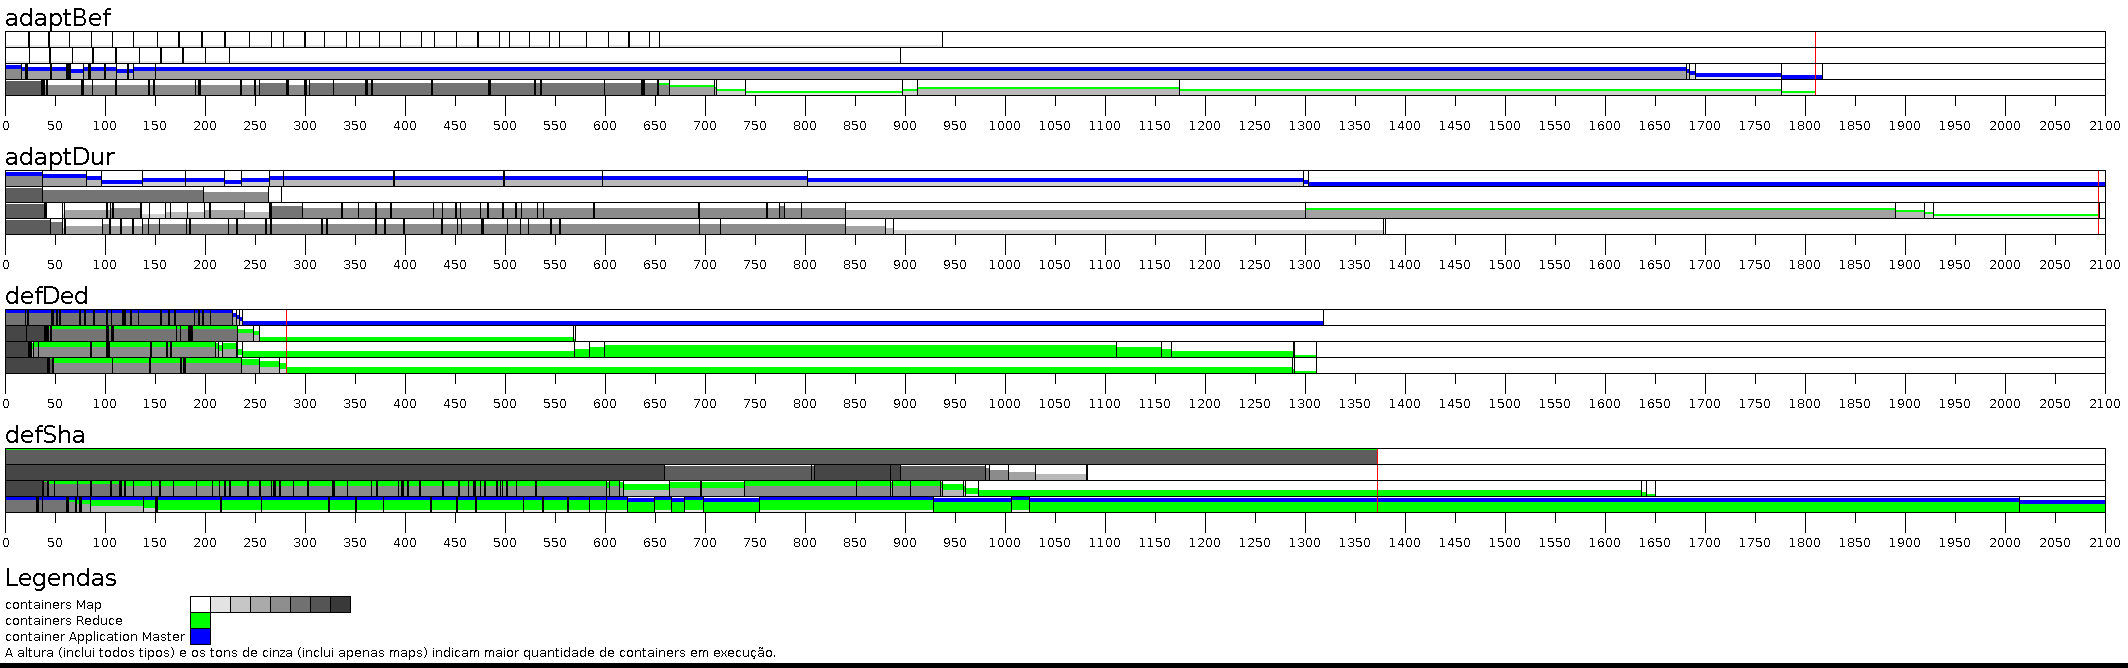
\includegraphics[width=1\textwidth]{figuras/TS-real.png}
	\caption{Diagrama de Gantt para os experimentos reais com TeraSort}
	\label{fig:exp2TS}
\end{figure}

\begin{figure}[!ht]
	\centering
	\includegraphics[height=15cm]{figuras/DFSIO-real.png}
	\caption{Diagrama de Gantt para os experimentos reais com TestDFSIO}
	\label{fig:exp2IO}
\end{figure}

\begin{figure}[!ht]
	\centering
	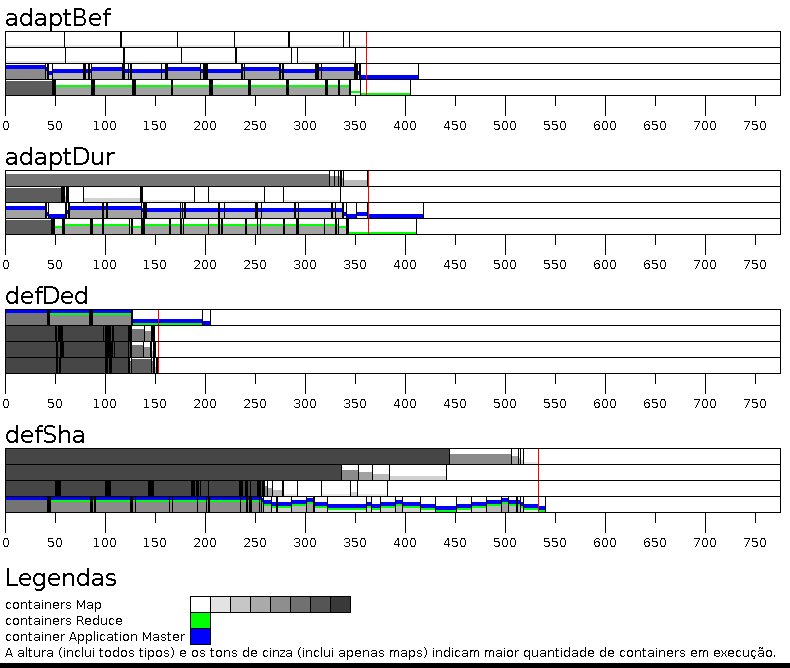
\includegraphics[height=15cm]{figuras/WC-real.png}
	\caption{Diagrama de Gantt para os experimentos reais com WordCount}
	\label{fig:exp2WC}
\end{figure}


\section{Experimento de escala}
Uma vez que os experimentos anteriores já responderam algumas questões importantes sobre a viabilidade da solução implementada, este experimento foi realizado com objetivo de analisar se as melhorias no escalonamento são mantidas quando o Hadoop é utilizado em um ambiente ou com uma entrada de dados maior. O experimento utiliza a solução descrita no Capítulo \ref{cap:desen}. A situação expressada com este experimento é de quando os nós do \textit{cluster} começam a ser utilizados por outros usuários antes/durante a aplicação \textit{MapReduce}.

\subsection{Procedimentos}
Neste experimento buscou-se analisar o comportamento da solução em um ambiente compartilhado de maior escala que nos experimentos anteriores. Foram feitos 2 experimentos distintos, um com escala de aplicação outro com escala de ambiente. Para a escala de aplicação a única diferença das configurações foi o tamanho da entrada, sendo utilizada uma entrada de 30 Gb para o TeraSort. Para a escala de ambiente, utilizou-se um \textit{cluster} com X escravos, sendo que a proporção de recursos reduzidos/livres continuou a mesma. 

\subsection{Resultados e Interpretações}

